%!TEX root = ../main.tex

\section*{Results}

  There is significant variation both in the networks as well as the \ac{otu}/\ac{esv} tables when different combinations of methods are used to generate them.
  Figure \ref{fig:otu_correlations} shows the comparison of several denoising and clustering methods.
  The data shows that all the methods that perform either clustering or denoising are highly correlated with each other.
  The correlation is low when comparing a method that performs clustering on the sequences with a method that performs denoising (Figure \ref{fig:otu_correlations}).
  The common core network (network made up of edges that are predicted by all methods) is very small compared to the total number of edges predicted by all the methods (Figure \ref{fig:denoise_network}).
  In this result, only the denoising method was changed (database used: \ac{gg} and network inference: \ac{sparcc}).
  But, nonetheless this approach of identifying a common network will help identify links with a good degree of confidence.

  SILVA and \ac{gg} are two popular 16S databases used for taxonomy identification.
  The two databases vastly differ in terms of their last update status - \ac{gg} was last updated on May 2013 and SILVA was last updated on December 2017.
  Since updates to taxonomic classifications are frequent, these two databases vary significantly \cite{Balvociute2017}.
  As a consequence of this, when different taxonomy databases are used on the same data-set we see large numbers of misclassifications \ref{fig:tax_mismatches}.

  Different network inference methods infer significantly different association networks.
  We can divide the network inference methods into two sets, the first set of methods (Pearson, Spearman, \ac{sparcc}) infer pairwise correlations while the second set infer direct associations (\ac{spieceasi}, \ac{mldm}, \ac{daa}).
  Our preliminary analysis (Figure \ref{fig:network_comparison}) shows that networks generated using 4 different methods (Pearson, Spearman, \ac{sparcc}, \ac{spieceasi}) are vastly different and the degree of similarity (number of edges that overlapped) between the methods was dependent on the data-set used.
  The abundance profiles of the different data-sets used are show in Figure \ref{fig:abundance_profile}.

  The pipeline and the data visualization tool help the user explore the effect of the various methods on their data.
  Exploring these differences are difficult and inconvenient without the tool since different tools differ in their input and output formats and require inter-converting between the various formats.
  In the case of our pipeline, this is handled automatically.

  \begin{figure}[h]
    \begin{center}
      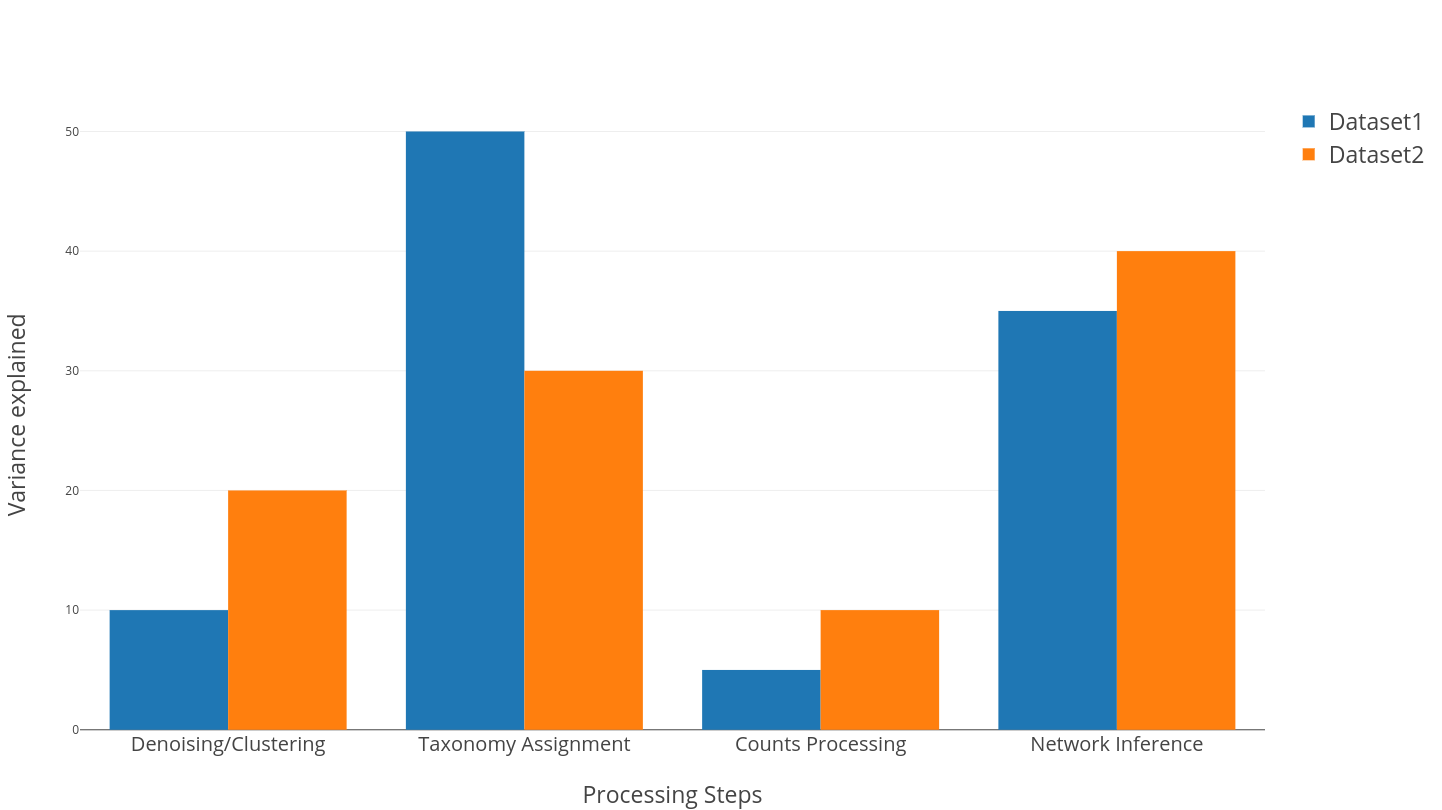
\includegraphics[width=17.8cm]{main_figure.png}
      \caption{\textbf{Percentage of variance in the final co-occurrence network due to each processing step.} }
      \label{fig:variance}
    \end{center}
  \end{figure}

  \begin{figure}[h]
    \begin{center}
      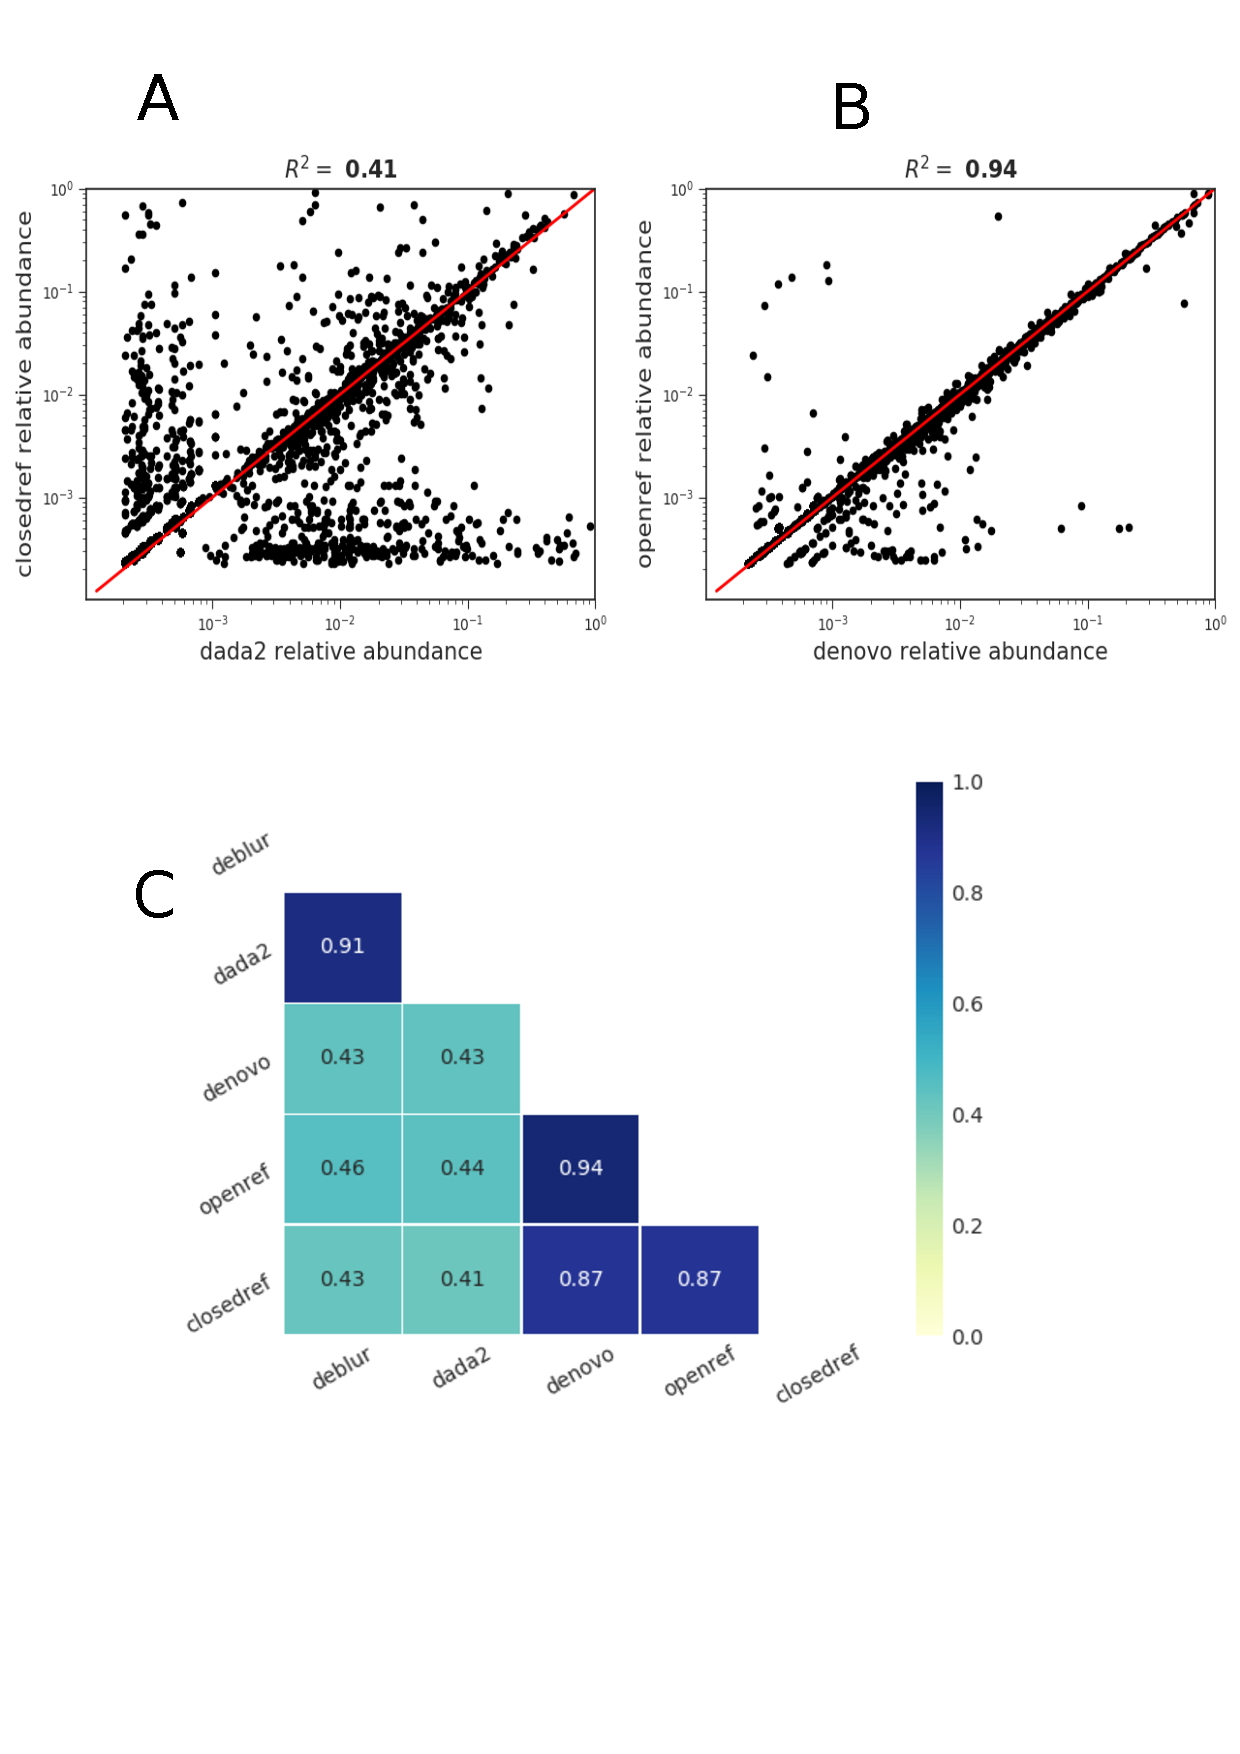
\includegraphics[width=15.8cm]{otu_corr_full.pdf}
      \caption{
        \textbf{Comparison of various denoising and clustering algorithms used in the pipeline}.
        (A, B) Correlation of the abundances of the taxa that are common between the count matrices created by two different methods.
        (A) The best correlation (most similar methods) is between open-reference and denovo.
        (B) The worst correlation (least similar methods) is between open-reference and dada2.
        (C) A heatmap showing the $\mathrm{R}^2$ of all pairwise comparisons of the methods.
      }
      \label{fig:otu_correlations}
    \end{center}
  \end{figure}

  \begin{figure}[h]
    \begin{center}
      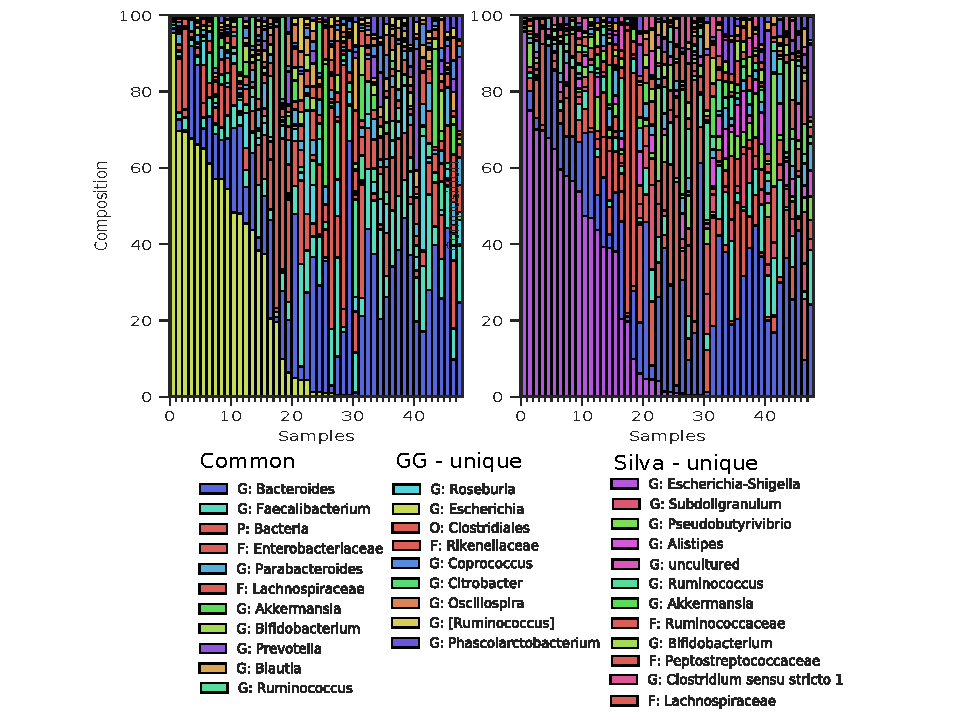
\includegraphics[width=17.8cm]{tax_comp_full.pdf}
      \caption{\textbf{Taxonomy composition of the 20 most abundant genera predicted using different taxonomy references databases}. NOTE: I will replace the legend with the taxonomy tree}
      \label{fig:tax_comparison}
    \end{center}
  \end{figure}

  \begin{figure}[h]
    \begin{center}
      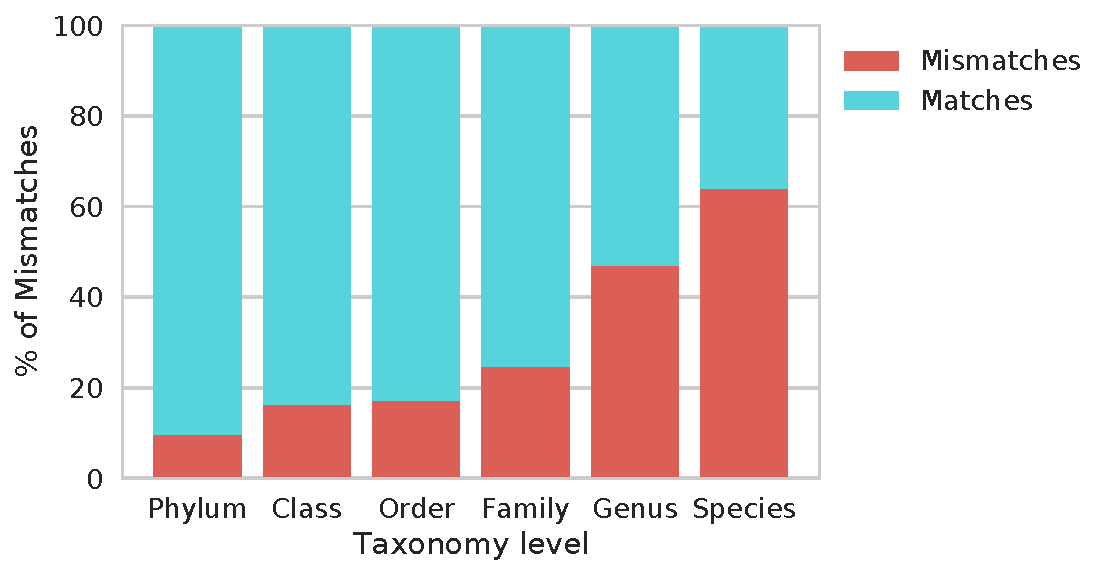
\includegraphics[width=15.8cm]{tax_distance_deblur.pdf}
      \caption{\textbf{Average percentage of mismatches in taxonomy assignment at various taxonomy levels}. NOTE: I will include a boxplot of the weighted distance in the taxonomy tree}
      \label{fig:tax_mismatches}
    \end{center}
  \end{figure}

  \begin{figure}[h]
    \begin{center}
      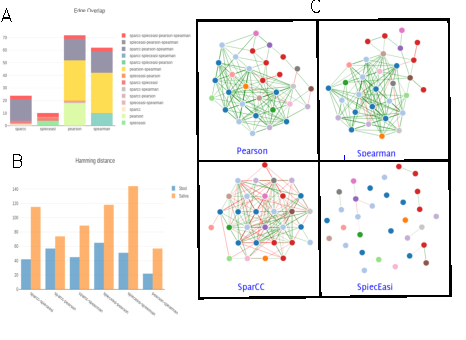
\includegraphics[width=17.8cm]{net_inference_comparison.pdf}
      \caption{
        \textbf{Networks generated using different network inference methods}.
        The four different networks generated by different network inference methods are very dissimilar (C).
        (A) The overlaps between the edges among the network5 generated is shown. The number of edges that are common to all networks are very low (5).
        (B) The hamming distance between the networks is shown. The similarity between various methods was found to vary with the data-source used.
      }
      \label{fig:network_comparison}
    \end{center}
  \end{figure}


  \begin{figure}[h]
    \begin{center}
      %\includegraphics[width=17.8cm]{../figures/network_comparison.pdf}
      \caption{\textbf{Core network captures known interactions in vaginal microbiota.} \textbf{a} Core network, obtained by taking the intersection between all the different pipelines. \textbf{b} Vaginal microbiota network as determined by XXX.}
      \label{fig:real_network}
    \end{center}
  \end{figure}
